\section{Numerical Analysis}
\label{sec:signature-numerical}

This section presents a numerical analysis of the signature-based framework for curve classification. We define the use of the logarithmic signature for classifying curves, introduce a distance metric to compare the signatures of two curves, and employ this metric for classification purposes.

\subsection{Distance Metric for Logarithmic Signatures}
\label{subsec:distance-metric-signature}

The distance metric for comparing the logarithmic signatures of two curves \(c_1\) and \(c_2\) is defined as follows:

\begin{equation}
    d_{\text{sig}_*}(c_1, c_2) = \left\| \frac{\mathcal{LS}(c_1^*)}{\|\mathcal{LS}(c_1^*)\|_2} - \frac{\mathcal{LS}(c_2^*)}{\|\mathcal{LS}(c_2^*)\|_2} \right\|_2,
    \label{eq:signature-distance-metric}
\end{equation}
where \(\mathcal{LS}(c_i^*)\) denotes the logarithmic signature of the curve \(c_i\), adjusted to start at the identity by transforming all elements using the inverse of the first element. The signatures are normalized by their \(L^2\) norm to ensure a standardized comparison. It should be noted that this choice is based on empirical observations and not theoretical reasons, which is a topic for future research.

We utilize the iisignature library \cite{reizensteinIisignatureLibraryEfficient2018}, which implements logarithmic signature computations using the Lyndon basis. Although it is possible to use the Hall basis, we chose the Lyndon basis due to its superior results.

\subsection{Impact of Truncation on Curve Distances}
\label{subsec:truncation-curve-distances-signature}

This section explores the effects of truncation on curve distances and the transition from continuous to discrete settings when using logarithmic signatures. This analysis provides insights into the practical application of logarithmic signatures for data analysis.

Utilizing the iisignature package, we examine logarithmic signatures framed in the Lyndon basis, as detailed in \cite{reizensteinCalculationIteratedIntegralSignatures2017}. For a triadic letter set, the Lyndon basis is tabulated in Table~\ref{tab:log_signatures}.

\begin{table}
    \centering
    \begin{tabular}{|c|c|c|c|}
    \hline
    \textbf{N} & \textbf{Level} & \textbf{\( u \)} & \textbf{\( \sigma(u) \)} \\
    \hline
    1 & 1 & 1 & \([1]\) \\
    2 & 1 & 2 & \([2]\) \\
    3 & 1 & 3 & \([3]\) \\
    \hline
    4 & 2 & 12 & \([1, 2]\) \\
    5 & 2 & 13 & \([1, 3]\) \\
    6 & 2 & 23 & \([2, 3]\) \\
    \hline
    7 & 3 & 112 & \([1,[1,2]]\) \\
    8 & 3 & 113 & \([1,[1,3]]\) \\
    9 & 3 & 122 & \([[1,2],2]\) \\
    10 & 3 & 123 & \([1,[2,3]]\) \\
    11 & 3 & 132 & \([[1,3],2]\) \\
    12 & 3 & 133 & \([[1,3],3]\) \\
    13 & 3 & 223 & \([2,[2,3]]\) \\
    14 & 3 & 233 & \([[2,3],3]\) \\
    \hline
    \multicolumn{4}{|c|}{\vdots} \\
    \hline
    \end{tabular}
    \caption{The Lyndon words consisting of three letters, up to truncation level 3, and their images under the permutations \(\sigma\).}
    \label{tab:log_signatures}
\end{table}

The dimensionality of truncated logarithmic signatures, dependent on truncation level \( n \) and dimension \( d \), is computed using Witt's formula, essential in free Lie algebra dimensional analysis \cite{metropolisWittVectorsAlgebra1983}. Witt's formula is given by:

\begin{equation}
    W(d, n) = \sum_{l=1}^{n} \frac{1}{l} \sum_{x | l} \mu\left(\frac{l}{x}\right) d^x,
\end{equation}
where \( \mu \) represents the Möbius function \cite{delegliseComputingSummationMobius1996}:

\begin{equation}
    \mu(n) = 
    \begin{cases} 
        +1 & \text{if } n \text{ is square-free with an even number of prime factors}, \\
        -1 & \text{if } n \text{ is square-free with an odd number of prime factors}, \\
        0 & \text{if } n \text{ has a squared prime factor}.
    \end{cases}
\end{equation}

Table~\ref{tab:dimensionality} presents the dimensions of truncated log signatures at various levels for a word length of three.

\begin{table}
    \centering
    \begin{tabular}{|c|c|c|c|c|c|c|c|c|}
    \hline
    \textbf{\( n \)} & \textbf{1} & \textbf{2} & \textbf{3} & \textbf{4} & \textbf{5} & \textbf{6} & \textbf{7} & \(\cdots\)\\
    \hline
    \textbf{d = 3} & 3 & 6 & 14 & 32 & 80 & 196 & 508 & \(\cdots\)\\
    \hline
    \end{tabular}
    \caption{Dimensionality of the logarithmic signature at different truncation levels}
    \label{tab:dimensionality}
\end{table}

We observe that the distance between logarithmic signatures increases with higher truncation levels. For signatures at levels \( i \) and \( i+1 \), this can be expressed as:
\begin{equation}
\|\mathcal{LS}(x_{i+1}) - \mathcal{LS}(y_{i+1})\| \geq \|\mathcal{LS}(x_i) - \mathcal{LS}(y_i)\| + \| \text{Terms at } i+1 \|,
\label{eq:distance_truncation}
\end{equation}
where \( \mathcal{LS}(x_i) \) and \( \mathcal{LS}(y_i) \) are logarithmic signatures at level \( i \), and \( \mathcal{LS}(x_{i+1}) \) and \( \mathcal{LS}(y_{i+1}) \) are at level \( i+1 \). This means that when we include more terms in the logarithmic signature (by increasing the truncation level), the distance between the signatures of two different paths either stays the same or becomes larger.

Future work could explore the existence of a scaling factor to enable the comparison of distances between different truncation levels.

%%%%%%%%%%%%%%%%%%%%%%%%%%%%%%%%%%%%%%%%%%%%%%%%%%%%%%%%%%%%%

\subsection{Classification of Curves}
\label{subsec:classification-curves-signature}

This subsection aims to classify curves based on their geometric characteristics utilizing a signature-based framework. The approach utilizes synthetic data, as discussed in Subsection \ref{subsec:synthetic-data-generation}, and employs methodologies outlined in prior analyses for curve generation. These curves are produced according to the procedures specified in Subsection \ref{subsec:reparameterization-curves}, for transformations in \(\mathrm{SO}(3)\), \(\mathrm{SE}(3)\), \(\mathrm{SO}(3)^3\), and \(\mathrm{SE}(3)^3\) spaces, respectively.

We employ the shape space metric \(d_{\text{sig}_*}\) (Equation \eqref{eq:signature-distance-metric}) to compute distances between each pair of curves, leading to the construction of a distance matrix. Currently, we have not addressed the scalar difference between the Frobenius norm and the \(2\)-norm of the vector format for curves in \(\mathrm{SE}(3)\) (Section \ref{sec:curves-in-SE3}), which may cause the method to focus excessively on translation. Visualizing this matrix with a color map facilitates the interpretation of these distances, where color intensity is inversely proportional to the geometric similarity between curves.

A key anticipated outcome is the formation of a block diagonal pattern within the distance matrix. This pattern is expected to manifest as three distinct 4x4 blocks along the diagonal, each block representing lower distances indicative of shape similarities. Conversely, off-diagonal blocks should display higher, relatively uniform distances, highlighting the presence of distinct geometric shapes. Such a configuration would underscore the efficacy of the signature-based classification method, confirming that curves sharing geometric properties cluster together in the shape space, while distinctly different shapes are effectively segregated.

\begin{figure}
    \centering
    \begin{subfigure}{0.48\textwidth}
        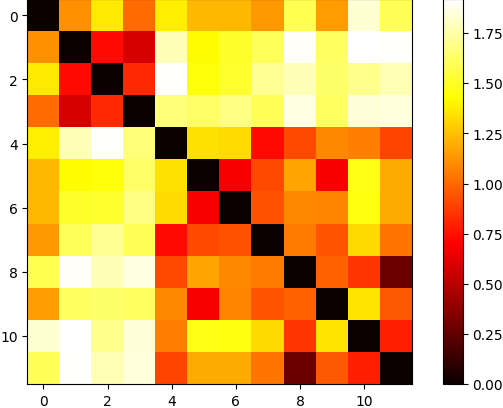
\includegraphics[width=\linewidth]{figures/syntetic_data/distance_matrix/SO3_signature_3.png}
        \caption{}
        \label{fig:classification-signature-level3-SO3}
    \end{subfigure}
    \hfill
    \begin{subfigure}{0.48\textwidth}
        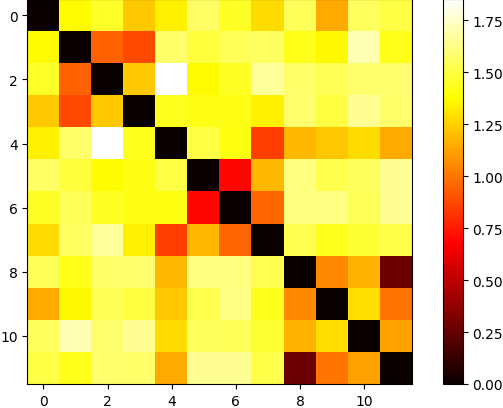
\includegraphics[width=\linewidth]{figures/syntetic_data/distance_matrix/SO3_signature_5.png}
        \caption{}
        \label{fig:classification-signature-level5-SO3}
    \end{subfigure}
    \vskip\baselineskip
    \begin{subfigure}{0.48\textwidth}
        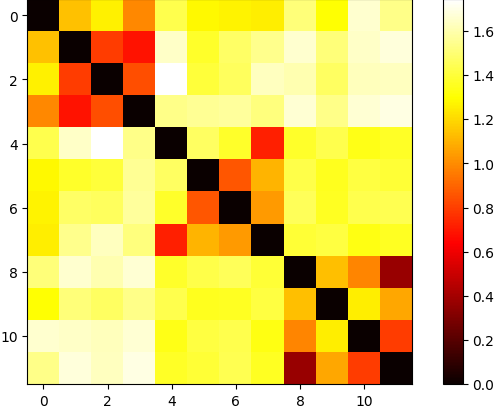
\includegraphics[width=\linewidth]{figures/syntetic_data/distance_matrix/SE3_signature_3.png}
        \caption{}
        \label{fig:classification-signature-level3-SE3}
    \end{subfigure}
    \hfill
    \begin{subfigure}{0.48\textwidth}
        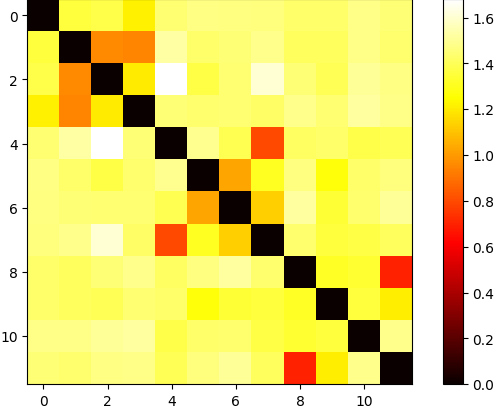
\includegraphics[width=\linewidth]{figures/syntetic_data/distance_matrix/SE3_signature_5.png}
        \caption{}
        \label{fig:classification-signature-level5-SE3}
    \end{subfigure}
    \caption[Classification using logarithmic signature on curves in \(\mathrm{SO}(3)\) and \(\mathrm{SE}(3)\)]{Distance matrices using the signature method for \(\mathrm{SO}(3)\) and \(\mathrm{SE}(3)\) at different truncation levels, visualized through the \(L^2\) norm between normalized signatures. Panels: (a) \(\mathrm{SO}(3)\), truncation level 3; (b) \(\mathrm{SO}(3)\), truncation level 5; (c) \(\mathrm{SE}(3)\), truncation level 3; (d) \(\mathrm{SE}(3)\), truncation level 5. These matrices illustrate the variation in signature-based classification accuracy across truncation levels.}
    \label{fig:classification-signature}
\end{figure}

\begin{figure}
    \centering
    \begin{subfigure}{0.48\textwidth}
        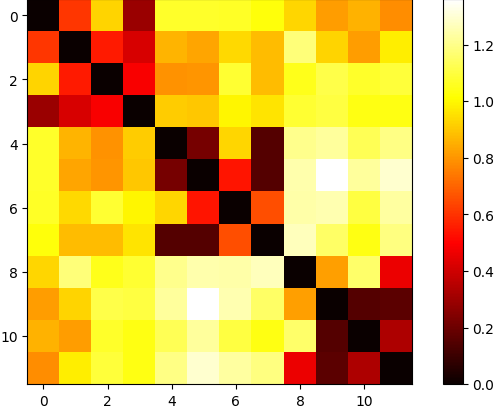
\includegraphics[width=\linewidth]{figures/syntetic_data/distance_matrix/SO3_3_signature_3.png}
        \caption{}
        \label{fig:classification-signature-level3-SO3-3}
    \end{subfigure}
    \hfill
    \begin{subfigure}{0.48\textwidth}
        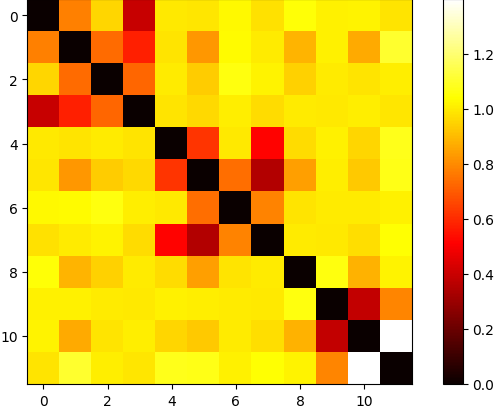
\includegraphics[width=\linewidth]{figures/syntetic_data/distance_matrix/SO3_3_signature_5.png}
        \caption{}
        \label{fig:classification-signature-level5-SO3-3}
    \end{subfigure}
    \vskip\baselineskip
    \begin{subfigure}{0.48\textwidth}
        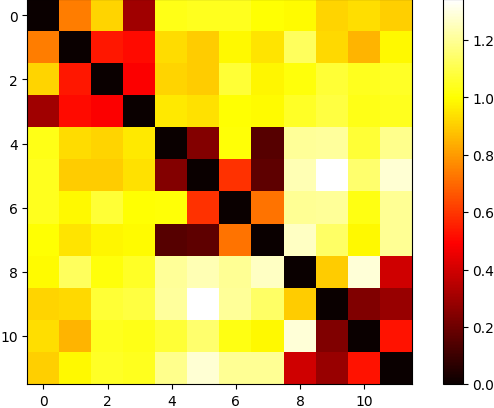
\includegraphics[width=\linewidth]{figures/syntetic_data/distance_matrix/SE3_3_signature_3.png}
        \caption{}
        \label{fig:classification-signature-level3-SE3-3}
    \end{subfigure}
    \hfill
    \begin{subfigure}{0.48\textwidth}
        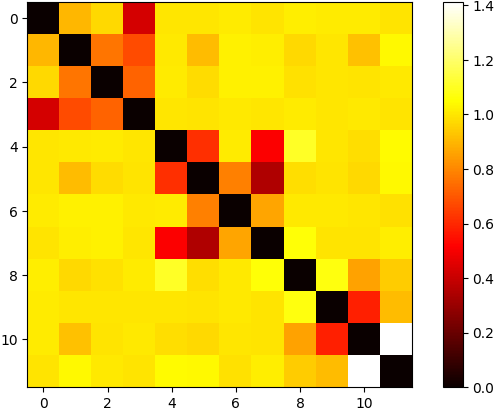
\includegraphics[width=\linewidth]{figures/syntetic_data/distance_matrix/SE3_3_signature_5.png}
        \caption{}
        \label{fig:classification-signature-level5-SE3-3}
    \end{subfigure}
    \caption[Classification using logarithmic signature on in \(\mathrm{SO}(3)^n\) and \(\mathrm{SE}(3)^n\)]{Distance matrices using the signature method for \(\mathrm{SO}(3)^3\) and \(\mathrm{SE}(3)^3\) at different truncation levels, visualized through the \(L^2\) norm between normalized signatures. Panels: (a) \(\mathrm{SO}(3)^3\), truncation level 3; (b) \(\mathrm{SO}(3)^3\), truncation level 5; (c) \(\mathrm{SE}(3)^3\), truncation level 3; (d) \(\mathrm{SE}(3)^3\), truncation level 5. These matrices illustrate the variation in signature-based classification accuracy across truncation levels.}
    \label{fig:classification-signature-3}
\end{figure}

In Figure \ref{fig:classification-signature}, it is evident that \(\mathrm{SE}(3)\) curves are more readily classified compared to \(\mathrm{SO}(3)\) curves, as shown by the more distinct clustering observed within the same geometric types. Increasing truncation levels in \(\mathrm{SO}(3)\) generally improves classification accuracy by incorporating more detailed information, resulting in a tighter grouping of curves with similar geometric characteristics. However, an interesting observation is made when the truncation level in \(\mathrm{SE}(3)\) is increased to 5: some curves from the same shape space unexpectedly exhibit large distances between them.

Figure \ref{fig:classification-signature-3} highlights the classification results for the spaces \(\mathrm{SO}(3)^n\) and \(\mathrm{SE}(3)^n\), which are notably promising. Distances within the same shape space remain low, indicating effective classification. Interestingly, classification performs better in \(\mathrm{SE}(3)^n\) than in \(\mathrm{SO}(3)^n\), demonstrating a superior ability to resolve geometric differences in these extended spaces. Similar to \(\mathrm{SE}(3)\), when the truncation level is increased to 5 in both \(\mathrm{SO}(3)^n\) and \(\mathrm{SE}(3)^n\), some curves from the same shape space begin to show significant distances between them.

These results highlight that the logarithmic signature is capable of distinguishing between curves of different shapes. By combining this with post-processing techniques, such as clustering, it may be possible to determine the shape of a curve based on its signature. However, the results also indicate that the choice of truncation level is crucial, as increasing the level may lead to unexpected results. Future work could explore the optimal truncation level for curve classification using the signature-based framework.

\subsection{Perturbation Analysis}
\label{subsec:perturbation-analysis-signature}

In this subsection, we investigate how the logarithmic signature-based distance metric (Equation \eqref{eq:signature-distance-metric}) behaves under perturbations. We utilize the curves \(c_i^\text{eq}\) and \(c_{i,i+1,i+2}^\text{eq}\) created in Subsection \ref{subsec:synthetic-data-generation}. To create a perturbed version of these curves, we solve the same differential equation \eqref{eq:diff-eq-synthetic}, but with timesteps perturbed by adding small, normally distributed noise. This results in the perturbed curves \(c_i^\epsilon\) and \(c_{i,i+1,i+2}^\epsilon\), with \(i \in \{1,2,3\}\) and \(i \in \{1,4,7\}\), respectively. We examine the effect of this perturbation on the signature-based distance metric by progressively reducing the standard deviation of the noise, performing this reduction 10 times. The results are shown in Figure \ref{fig:perturbation-analysis-signature}.

\begin{figure}
    \centering
    \begin{tikzpicture}
        \begin{loglogaxis}[
            width=0.8\textwidth,
            height=0.4\textwidth,
            xlabel={\(\epsilon\)},
            ylabel={\(d_{\mathcal{\text{sig}}_*}(c^\epsilon, c)\)},
            legend style={font=\small, at={(1.2,0.5)}, anchor=west},
            grid=major,
            legend pos=outer north east,
        ]
        
        \addplot [thick, red, solid] table [x=perturbation, y=c1, col sep=comma] {figures/syntetic_data/perturbation-analysis/signature-SO3.csv};
        \addlegendentry{\(\omega_0\)}

        \addplot [thick, blue, solid] table [x=perturbation, y=c2, col sep=comma] {figures/syntetic_data/perturbation-analysis/signature-SO3.csv};
        \addlegendentry{\(\omega_1\)}

        \addplot [thick, green, solid] table [x=perturbation, y=c3, col sep=comma] {figures/syntetic_data/perturbation-analysis/signature-SO3.csv};
        \addlegendentry{\(\omega_2\)}

        \addplot [thick, red, dashed] table [x=perturbation, y=c1, col sep=comma] {figures/syntetic_data/perturbation-analysis/signature-SE3.csv};
        \addlegendentry{\(\xi_0\)}

        \addplot [thick, blue, dashed] table [x=perturbation, y=c2, col sep=comma] {figures/syntetic_data/perturbation-analysis/signature-SE3.csv};
        \addlegendentry{\(\xi_1\)}

        \addplot [thick, green, dashed] table [x=perturbation, y=c3, col sep=comma] {figures/syntetic_data/perturbation-analysis/signature-SE3.csv};
        \addlegendentry{\(\xi_2\)}

        \logLogSlopeTriangle{0.7}{0.3}{0.2}{1}{black, dashed}
        
        \end{loglogaxis}
    \end{tikzpicture}
    \caption[Perturbation analysis plot of the logarithmic signature distance]{The signature based distance metric under perturbations in \(\mathrm{SO}(3)\) and \(\mathrm{SE}(3)\). The distance between the perturbed and non-perturbed curves is computed using the signature based distance metric. The curves are perturbed by adding a small normal distributed noise to the parameterization, where we halve the standard deviation, and the distance is computed 10 times.}
    \label{fig:perturbation-analysis-signature}
\end{figure}

We observe that as the perturbation size decreases, the signature-based distance metric also decreases. This indicates that the metric is robust to small perturbations, maintaining consistent performance even with minor noise in the parameterization of the curves.